% SPDX-License-Identifier: Apache-2.0
%
% A network on chip in TxHDL. Built by //docs:noc. Every listing is
% included from the tree.
\documentclass[journal,9pt]{IEEEtran}

% Listings of Rust set by rustfmt at 80 columns: 5.6pt is what fits
% the frame of a column (issue 1061).
\newcommand{\listingsize}{\fontsize{5.6}{6.6}\selectfont}
% SPDX-License-Identifier: Apache-2.0
%
% The house preamble, shared by every document in this directory. Loaded
% after \documentclass, before \title. Keeping it in one file is what
% stops two articles drifting apart in font, listing style or figure
% style.
% Computer Modern. IEEEtran selects Times (ptm) by default, so the face has
% to be chosen explicitly.
%
% Latin Modern is the Computer Modern variety used here, and the choice is
% forced rather than aesthetic. Under T1 encoding, plain `cmr` has no Type 1
% outlines unless cm-super is installed, and it is not in the pinned
% distribution, so pdflatex falls back to EC bitmaps and every glyph in the
% PDF becomes a Type 3 font. That was measured: the first build produced a
% document with 10 Type 3 fonts and no Type 1. Latin Modern is Computer
% Modern redrawn with a full T1 repertoire and real .pfb outlines, so the
% same design comes out scalable.
\usepackage[T1]{fontenc}
\usepackage[utf8]{inputenc}
\usepackage{lmodern}
% microtype is not in the pinned TeX distribution. emergencystretch alone
% keeps the two-column measure from producing overfull lines.
\setlength{\emergencystretch}{3em}

\usepackage{amsmath}
\usepackage{amssymb}
\usepackage{amsthm}
\usepackage{booktabs}
\usepackage{array}
% enumitem is not in the pinned TeX distribution; the list spacing below
% does what \setlist would have done.
\usepackage{float}
\usepackage{xcolor}
\usepackage{listings}
\usepackage{tikz}
\usetikzlibrary{arrows.meta,positioning,fit,backgrounds,calc}
\usepackage[hidelinks,bookmarks=true]{hyperref}

% Numbered, definition-style box for a rule the reader is meant to apply.
\theoremstyle{definition}
\newtheorem{rulebox}{Rule}
\newtheorem{example}{Example}

% Unnumbered asides.
\theoremstyle{remark}
\newtheorem*{tip}{Tip}
\newtheorem*{pitfall}{Pitfall}

% Tighter lists, in place of enumitem's \setlist.
\setlength{\topsep}{2pt}
\setlength{\itemsep}{1pt}
\setlength{\parsep}{0pt}

% Code in the running text. The typewriter face under T1 ligates `<<`
% and `>>` into guillemets, so a shift printed as \code{<<} came out as
% a French quotation mark (issue 571). microtype's \DisableLigatures is
% not in the pinned distribution, but the primitive it rests on is
% pdfTeX's own: \pdfnoligatures strips every ligature from the font it
% is given, and the current font inside \texttt is the typewriter face
% at the size in use, so each size is stripped the first time \code
% sets it. Code wants no ligature at all: two quotes are two quotes.
\newcommand{\code}[1]{\texttt{\ifdefined\pdfnoligatures\pdfnoligatures\font\fi #1}}
\newcommand{\term}[1]{\emph{#1}}

% Syntax highlighting. Four roles, distinguishable in colour and still
% distinguishable in greyscale, because an IEEE article gets printed: the
% keyword is the only bold role, the comment is the only italic one, and the
% two remaining roles differ in lightness as well as in hue.
\definecolor{kwblue}{RGB}{20,60,150}
\definecolor{cmtgreen}{RGB}{90,120,90}
\definecolor{strred}{RGB}{150,50,40}
\definecolor{numgray}{gray}{0.45}
\definecolor{framegray}{gray}{0.70}
\definecolor{bgshade}{gray}{0.97}
% A darker fill for figure cells. The listing background has to stay very
% light to keep code readable; a figure cell has to be clearly shaded or the
% distinction it draws is invisible in print.
\definecolor{cellshade}{gray}{0.90}

% The listing size is the document's choice, because it depends on the
% column: a two-column article sets `\listingsize` to 6pt and keeps its
% listings within 70 columns, or to 5.6pt when it includes source that
% rustfmt sets at 80, which is what fits a column's frame (issue 1061);
% a one-column document keeps the body size and includes source files
% at 80. `//docs:frame_test` checks every listing line against its frame. Lines are never broken; a line that does not fit
% overflows the frame, which is visible, rather than wrapping, which is
% not.
\providecommand{\listingsize}{\scriptsize}

% `'` is deliberately not a string delimiter: the language uses it for loop
% labels, as Rust does, so treating it as a quote would swallow the rest of
% the line.
\lstdefinestyle{txhdl}{
  basicstyle=\ttfamily\listingsize,
  keywordstyle=\bfseries\color{kwblue},
  commentstyle=\itshape\color{cmtgreen},
  stringstyle=\color{strred},
  numberstyle=\tiny\color{numgray},
  morekeywords={mod,use,pub,const,type,struct,enum,trait,impl,fn,async,let,mut,
    match,if,else,loop,while,for,in,break,continue,return,as,await,
    module,bus,channel,transaction,protocol,pipeline,flow,seq,config,
    port,stage,pipe,instance,connect,bind,tag,domain,blackbox,foreign,
    property,role,signal,handler,true,false,
    sequence,interface,modport,implements,package,import,var,wire,func,proc,
    case,default,next,fork,branch,join,state,fsm},
  morecomment=[l]{//},
  morestring=[b]",
  showstringspaces=false,
  columns=fullflexible,
  keepspaces=true,
  breaklines=false,
  % Framed, so a listing is bounded rather than floating in the column.
  frame=single,
  rulecolor=\color{framegray},
  framesep=3pt,
  backgroundcolor=\color{bgshade},
  xleftmargin=3pt,
  xrightmargin=3pt,
  aboveskip=6pt,
  belowskip=6pt,
  % Every listing is numbered and captioned, so it can be referred to by
  % number. `caption` without `float` numbers the listing and leaves it
  % where it was written, which is what a listing in running prose needs.
  captionpos=b,
  abovecaptionskip=2pt,
  belowcaptionskip=6pt,
}

% Figures drawn as text. Framed the same way, and with the highlighting
% switched off, because a box-and-arrow diagram is not code and half its
% words turning blue reads as an accident. Setting a style adds keys rather
% than clearing the ones already set, so the three roles are neutralised by
% hand rather than by leaving them out. Program output is printed in this
% style too, and a netlist's assignment can run past the frame, so a line
% that does not fit is broken and the rest indented; source never is.
\lstdefinestyle{ascii}{
  basicstyle=\ttfamily\listingsize,
  keywordstyle=\ttfamily,
  commentstyle=\ttfamily,
  stringstyle=\ttfamily,
  columns=fullflexible,
  keepspaces=true,
  breaklines=true,
  breakindent=2em,
  frame=single,
  rulecolor=\color{framegray},
  framesep=3pt,
  backgroundcolor=\color{bgshade},
  xleftmargin=3pt,
  xrightmargin=3pt,
  aboveskip=6pt,
  belowskip=6pt,
}
\lstset{style=txhdl}

% House TikZ styles. `shorten` lives on the arrow styles rather than on each
% arrow, so every arrow in the document gets the gap, including ones added
% later. TikZ clips a path at a node's border, so without it an arrowhead
% butts against the box with no gap at all. Keep `node distance` well above
% twice the shorten, or the arrow shrinks to nothing.
\tikzset{
  box/.style={draw,rounded corners=2pt,align=center,inner sep=4pt,
              font=\footnotesize},
  boxf/.style={box,fill=bgshade},
  lbl/.style={font=\scriptsize\itshape,align=center},
  fl/.style={-{Stealth[length=4pt]},shorten >=2.5pt,shorten <=2.5pt},
  fld/.style={fl,dashed},
}


% The contents list: the class gives a section's number 2.75em, which
% a Roman numeral past thirty overruns onto the title, so the box is
% wider here, and a subsection's entry starts where a title does.
\makeatletter
\def\l@section#1#2{\addpenalty{\@secpenalty}\addvspace{1.0em plus 1pt}%
    \@tempdima 5.75em \begingroup \parindent \z@ \rightskip \@pnumwidth%
    \parfillskip-\@pnumwidth {\bfseries\leavevmode #1}\hfil\hbox to\@pnumwidth{\hss #2}\par%
    \endgroup}
\def\l@subsection{\@dottedtocline{2}{5.75em}{5em}}
\def\l@subsubsection{\@dottedtocline{3}{10.75em}{5.5em}}
\makeatother

% SPDX-License-Identifier: Apache-2.0
% The boards' memory maps, written by //tools/memmap from the maps the
% designs decode (issue 444). A document asks for a table with
% \mmget{<what>}{<board>}, and a table the generator does not write
% stops the document rather than leaving a gap.
\input{tools/memmap/mm_tables}
\makeatletter
\newcommand{\mmget}[2]{%
  \@ifundefined{mm@#1@#2}%
    {\PackageError{memmap}{//tools/memmap writes no #1 for #2}%
      {Add it to tools/memmap/main.rs.}}%
    {\csname mm@#1@#2\endcsname}}
\makeatother

\usepackage{graphicx}

\InputIfFileExists{buildstamp.tex}{}{}
\providecommand{\buildstamp}{Draft build (outside the Bazel flow).}

% A range of a source file of the network, by its begin/end markers.
% A range of the system's source.
\newcommand{\socpart}[3]{%
\lstinputlisting[rangebeginprefix=//\ begin\{,rangebeginsuffix=\},%
rangeendprefix=//\ end\{,rangeendsuffix=\},includerangemarker=false,%
linerange=#1-#1,caption={#2},label={#3}]{soc/src/lib.rs}}

% A range of a source file of the network, by its begin/end markers.
\newcommand{\nocpart}[4]{%
\lstinputlisting[rangebeginprefix=//\ begin\{,rangebeginsuffix=\},%
rangeendprefix=//\ end\{,rangeendsuffix=\},includerangemarker=false,%
linerange=#2-#2,caption={#3},label={#4}]{lib/parts/src/bus/noc/#1}}

\title{A Network on Chip in TxHDL}

\author{Filip Filmar and Dragiša Janković%
\thanks{Both authors are independent. Filip Filmar is the
corresponding author, at f@hdlfactory.com; Dragiša Janković is
reached at linkedin.com/in/dragisa-jankovic.}%
\thanks{This is the tutorial on the network, for a reader who knows
the AXI link~\cite{axi} and wants more than one host and more than
one peripheral on it. Every listing is included from the project
repository \code{HDL/txhdl} at build time. The cover~\cite{cover}
lists every document.}%
\thanks{The authors used a large language model, Claude, as an
assistant in exploring the concepts and in writing and constructing
the documents and the programs; every commit of the repository says
so and records the prompts that led to it, verbatim.}%
\thanks{\buildstamp}}

\markboth{A Network on Chip in TxHDL}{Filmar and Janković: A Network on Chip in TxHDL}

\begin{document}
\maketitle

\begin{abstract}
A bus router connects multiple peripherals to a single host. In contrast,
a network on chip interconnects multiple hosts and peripherals across a
two-dimensional lattice, enabling arbitrary point-to-point communication.
Each network node maintains bidirectional links with its four cardinal
neighbors alongside a local exit port for attaching endpoints. Links
multiplex traffic across two independent virtual channels to prevent
protocol deadlock. The network routes packets using deterministic
dimension-order routing. Network bridges translate standard AXI4 channel
transactions into fixed-format packets. Host and peripheral clients interact
through standard AXI interfaces without awareness of the underlying
packet-switched topology.
\end{abstract}


\begin{figure}[htbp]
\centering
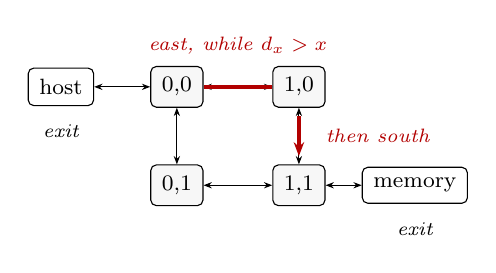
\begin{tikzpicture}[x=1.55cm, y=-1.25cm, font=\scriptsize]
  \node[boxf] (n00) at (0,0) {0,0};
  \node[boxf] (n10) at (1,0) {1,0};
  \node[boxf] (n01) at (0,1) {0,1};
  \node[boxf] (n11) at (1,1) {1,1};
  \draw[{Stealth[length=3pt]}-{Stealth[length=3pt]}] (n00) -- (n10);
  \draw[{Stealth[length=3pt]}-{Stealth[length=3pt]}] (n01) -- (n11);
  \draw[{Stealth[length=3pt]}-{Stealth[length=3pt]}] (n00) -- (n01);
  \draw[{Stealth[length=3pt]}-{Stealth[length=3pt]}] (n10) -- (n11);
  \node[box] (h) at (-0.95,0) {host};
  \node[box] (m) at (1.95,1) {memory};
  \draw[{Stealth[length=3pt]}-{Stealth[length=3pt]}] (h) -- (n00);
  \draw[{Stealth[length=3pt]}-{Stealth[length=3pt]}] (n11) -- (m);
  \draw[-{Stealth[length=5pt]}, very thick, red!70!black, shorten >=3pt,
        shorten <=3pt]
       (n00) -- (n10) -- (n11);
  \node[lbl, red!70!black] at (0.5,-0.42) {east, while $d_x > x$};
  \node[lbl, red!70!black, anchor=west] at (1.14,0.5) {then south};
  \node[lbl] at (-0.95,0.45) {exit};
  \node[lbl] at (1.95,1.45) {exit};
\end{tikzpicture}
\caption{A two-by-two lattice and the path a burst follows from the host
at (0,0) to the memory at (1,1). Dimension-order routing traverses X
first and then Y, preventing cyclic dependencies among network links.}
\label{fig:n-lattice}
\end{figure}

\section{Packet Framing}
\label{sec:n-pkt}

Figure~\ref{fig:n-lattice} illustrates the network topology. A physical link
transmits individual beats of an AXI channel, framed into packets targeted
to a coordinate node and stamped with their originating node identifier.

\nocpart{pkt.rs}{pkt}{Packet format definition.}{lst:n-pkt}

The packet structure maintains a uniform width matching the widest channel
beat, following the design principles of the Razboj instruction word~\cite{gpu}.
Lowered hardware requires fields at fixed bit offsets; variable-length headers
would necessitate serialization state machines across every port. A read
address beat clears payload and strobe fields to zero. A write response beat
clears address fields to zero. The \code{Chan} discriminant identifies the
active channel payload.

Packets encode return routing explicitly. Nodes maintain no internal state
tables for pending transactions; response packets route back to their origin
by inspecting the source coordinate embedded in the request.

\section{Virtual Channels}
\label{sec:n-vc}

Each link provides two dedicated virtual channels: one for requests and one
for responses. These channels operate over independent buffer queues without
shared storage. A network node instantiates two parallel switches, allocating
one to each virtual channel.

Physical separation guarantees deadlock freedom at the protocol level. A
peripheral processes an incoming request by generating an outbound response.
If saturated request queues could block response traffic, the responses
needed to retire pending requests could never traverse the fabric, resulting
in store-and-forward deadlock. Allocating an isolated channel to responses
guarantees forward progress regardless of request queue utilization.

\section{A Node}
\label{sec:n-node}

The network employs deterministic dimension-order routing. A packet advances
east or west until reaching the target column, traverses north or south to
reach the destination row, and exits through the local terminal port.

\begin{figure}[htbp]
\centering
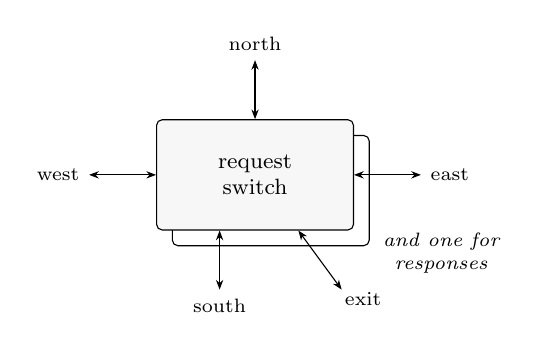
\begin{tikzpicture}[x=1cm, y=1cm, font=\scriptsize]
  % The response switch, behind: a node has two of these and they
  % share nothing.
  \node[box, fill=white, minimum width=2.5cm, minimum height=1.4cm]
       (p) at (0.2,-0.2) {};
  \node[lbl, anchor=north west] at (1.5,-0.62) {and one for\\responses};
  \node[boxf, minimum width=2.5cm, minimum height=1.4cm] (q) at (0,0)
       {request\\switch};
  % Each link leaves the side it is named for.
  \draw[{Stealth[length=3.5pt]}-{Stealth[length=3.5pt]}]
       (q.north) -- ++(0,0.75) node[above, font=\scriptsize] {north};
  \draw[{Stealth[length=3.5pt]}-{Stealth[length=3.5pt]}]
       ($(q.south)+(-0.45,0)$) -- ++(0,-0.75)
       node[below, font=\scriptsize] {south};
  \draw[{Stealth[length=3.5pt]}-{Stealth[length=3.5pt]}]
       (q.west) -- ++(-0.85,0) node[left, font=\scriptsize] {west};
  \draw[{Stealth[length=3.5pt]}-{Stealth[length=3.5pt]}]
       (q.east) -- ++(0.85,0) node[right, font=\scriptsize] {east};
  % The fifth port: where something that is not a node attaches.
  \draw[{Stealth[length=3.5pt]}-{Stealth[length=3.5pt]}]
       ($(q.south)+(0.55,0)$) -- ++(0.55,-0.75)
       node[below right, font=\scriptsize, inner sep=1pt] {exit};
\end{tikzpicture}
\caption{Switch architecture: four cardinal links and a fifth local exit
port. Each node instantiates two isolated switches per virtual channel to
prevent protocol deadlock. Host bridges inject requests and consume responses;
peripheral bridges invert this mapping.}
\label{fig:n-node}
\end{figure}

\nocpart{switch.rs}{route}{Dimension-order routing implementation.}{lst:n-route}

Restricting routing directions ensures deadlock freedom on two-dimensional
meshes. Because packets never turn from Y channels back onto X channels,
cyclic waiting chains cannot form across physical links.

A switch routes one packet per clock cycle. The router calculates target
directions and output buffer availability concurrently across all five
inputs, preventing blocked ports from stalling unblocked flows. An arbiter
schedules eligible packets using a round-robin policy. Inputs are ordered
cyclically: north, south, west, east, and exit. An internal \code{turn}
register tracks the starting priority index. The arbiter selects the first
eligible input at or following \code{turn}, updating the register to the
subsequent port. A serviced input moves to the end of the priority queue,
ensuring no packet waits behind more than four competing transfers.

\nocpart{switch.rs}{pick}{Round-robin arbiter rotations across \code{turn} states.}{lst:n-pick}

\nocpart{switch.rs}{run}{Cycle-by-cycle switch execution.}{lst:n-switch}

\nocpart{node.rs}{run}{Node definition containing dual virtual channel switches.}{lst:n-node}

\subsection{A lattice as one unit}
\label{sec:n-mesh}

Nodes receive their spatial coordinates via runtime inputs (\code{col} and
\code{row}) rather than compile-time generic types, unifying all network nodes
under a single concrete hardware type (issue 635). Instantiating logic binds
these coordinates to constants using \code{tie}. Synthesis tools propagate
these constants into address comparators, eliminating generic parameter
proliferation without silicon area penalty.

Using a uniform node type enables synthesizing the entire network mesh as a
single composite module. \code{Mesh<W, H, N, ..>} allocates \(N\) nodes
within a \code{Units} container, connecting node \(i\) at column \(i \pmod W\)
and row \(\lfloor i / W \rfloor\). Channel interconnects bind cardinal
directions across both virtual channels, exposing terminal exits as \(N\)-element
port arrays. Boundary links wrap toroidally to terminate open wires with
single drivers and receivers, though dimension-order routing never routes
traffic along wrap-around links. Explicit parameters define mesh dimensions
while const asserts verify that \(N = W \cdot H\). The test target \code{ex\_mesh}
synthesizes a 3 by 2 mesh, verifying netlist ports against simulation
traces~\cite{examples}.

\nocpart{mesh.rs}{mesh}{Lattice constructor wiring nodes as a composite unit.}{lst:n-mesh}

\section{The Exit}
\label{sec:n-bridge}

A network bridge connects standard AXI interfaces to packet-switched links
through host and peripheral adapters.

\begin{figure}[htbp]
\centering
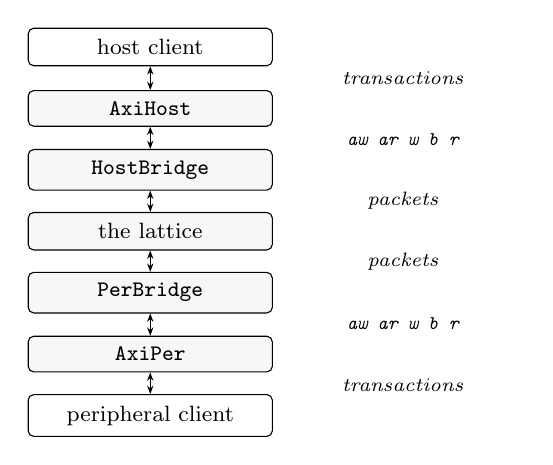
\begin{tikzpicture}[x=1cm, y=-0.78cm, font=\scriptsize,
                    every node/.style={minimum width=3.1cm}]
  \node[box] (hc) at (0,0) {host client};
  \node[boxf] (ht) at (0,1) {\code{AxiHost}};
  \node[boxf] (hb) at (0,2) {\code{HostBridge}};
  \node[boxf] (nw) at (0,3) {the lattice};
  \node[boxf] (pb) at (0,4) {\code{PerBridge}};
  \node[boxf] (pt) at (0,5) {\code{AxiPer}};
  \node[box] (pc) at (0,6) {peripheral client};
  \foreach \a/\b in {hc/ht,ht/hb,hb/nw,nw/pb,pb/pt,pt/pc}
    \draw[{Stealth[length=3pt]}-{Stealth[length=3pt]}] (\a) -- (\b);
  \node[lbl, anchor=west] at (1.65,0.5) {transactions};
  \node[lbl, anchor=west] at (1.65,1.5) {\code{aw ar w b r}};
  \node[lbl, anchor=west] at (1.65,2.5) {packets};
  \node[lbl, anchor=west] at (1.65,3.5) {packets};
  \node[lbl, anchor=west] at (1.65,4.5) {\code{aw ar w b r}};
  \node[lbl, anchor=west] at (1.65,5.5) {transactions};
\end{tikzpicture}
\caption{Protocol layers connecting endpoint clients across the network.
Standard AXI interfaces interact with protocol bridges that translate between
channel handshakes and network packets.}
\label{fig:n-layers}
\end{figure}

The host bridge encodes address beats into packets using a three-entry
address map. The final map entry specifies a default route with a zero mask,
directing unmatched addresses to a designated fallback node and eliminating
unroutable address exceptions.

Single-beat writes assemble into single packets containing both address and
data payloads. Multi-beat write bursts are decomposed by the host bridge:
the initial beat transmits with the address phase, while subsequent beats
dispatch as individual single-beat writes with incremented addresses. The
destination peripheral confirms each beat independently. The host bridge
aggregates these acknowledgments, returning a single response beat to the
master once all beats complete (emitting \texttt{SlvErr} if any beat faults).
This decomposition prevents write interleaving across single-ported
peripherals. Because AXI4 omits transaction identifiers on the write data
channel, interleaved beats from distinct masters would cause undetectable
data corruption. Decomposing bursts into atomic packets ensures that
individual writes complete without interruption.

Burst decomposition processes one burst at a time, holding subsequent
multi-beat writes until the active burst completes. Single-beat writes and
reads execute without blocking. Fixed bursts transmit all beats at a single
address. Wrapping bursts are rejected: the host bridge accepts the address
phase and data beats up to \code{wlast}, discards the transfer locally, and
returns \texttt{SlvErr} to maintain channel alignment.

\nocpart{bridge.rs}{hostrun}{Host bridge implementation.}{lst:n-host}

The peripheral bridge unpacks incoming packets into native AXI subordinate
channels and repacks responses for transmission back to the originating node.

The peripheral bridge also renames transaction identifiers. Because hosts
allocate identifiers independently, two masters may issue requests with
identical tags. To prevent response aliasing at shared peripherals, the
bridge translates incoming tags into a local identifier space while recording
the originating coordinate and host tag. Completion responses map back to the
original host tag and route to the source node. Tag availability bounds the
maximum number of concurrent in-flight transactions supported by the
peripheral.

\nocpart{bridge.rs}{perrun}{Peripheral bridge implementation.}{lst:n-per}

\section{What Is Checked}
\label{sec:n-tests}

The test suite in \code{noc.rs} comprises ten verification targets. Three
end-to-end integration tests instantiate four network nodes, both bridge
types, protocol trackers, and memory modules. The remaining unit tests
validate burst decomposition, wrapping burst rejections, and fair arbitration
across switch inputs.

The first integration test transmits bursts across the diagonal of a 2 by 2
mesh, exercising horizontal and vertical routing before verifying readback
integrity. The second test connects two hosts and a shared memory, verifying
that concurrent operations complete without tag aliasing.

The third test places four distinct peripherals behind a single node via an
AXI router. An exit port binds to one bridge, whose AXI interface drives a
four-port router with memory attached to each port. Two hosts write words
into every peripheral, read them back, and probe an unmapped address. The
router returns \code{DecErr} locally without deadlocking the network fabric.

\section{Four Corners}
\label{sec:n-soc}

\begin{figure}[htbp]
\centering
\includegraphics[width=0.52\columnwidth]{soc_scene.png}
\caption{Rendered icosahedron frame. The Vreteno processor computes vertex
transformations and populates display lists in shared memory; the Razboj
rasterizer fetches commands and renders pixels over the on-chip network.}
\label{fig:n-soc}
\end{figure}

The demonstration design deploys a 2 by 2 heterogeneous system: a Vreteno
processor core at (0,0), a Razboj rasterizer at (1,0), a shared RAM at (0,1),
and a UART controller at (1,1). Endpoints communicate solely across the
packet-switched fabric.

The two master cores interact through shared memory. The processor software
evaluates 3D icosahedron geometry, performs back-face culling, calculates
flat lighting, and writes display list primitives into memory at
\mmget{at}{soc_dl}, updating the command count at \mmget{at}{soc_count}.
The rasterizer detects the non-zero count, fetches command packets across the
network, and renders pixels into the framebuffer at \mmget{at}{soc_fb}.
Upon completion, the core emits confirmation over the serial port at
\mmget{at}{soc_serial}. Table~\ref{tab:n-map} summarizes the memory map.

\begin{table}[htbp]
\caption{System address map and network routing destinations.}
\label{tab:n-map}
\mmget{board}{soc}
\end{table}

\socpart{map}{Address map defined within the host bridge type.}{lst:n-map}

Address masks must cover the entire range. An address mask of \code{0xf000}
matches only the top nibble, causing alias addresses at \mmget{at}{soc_alias}
to misroute to the UART port, which emitted framebuffer bytes to the console
during early debugging.

Each corner integrates three components: the endpoint client, an \code{AxiHost}
or \code{AxiPer} engine, and the network bridge. The processor core required
no modifications to interface with the network fabric.

Running the system exposed a processor hazard: an integer multiply using
the result of an immediately preceding load sampled stale register data
because the load completion was still in flight on the bus. Adding pipeline
interlocks resolved the issue.

\section{What the Hops Cost}
\label{sec:n-cost}

\begin{table}[htbp]
\caption{Execution cycles for icosahedron rendering: direct link versus
network lattice.}
\label{tab:n-cost}
\centering\footnotesize
\begin{tabular}{@{}lrr@{}}
\toprule
 & link & lattice \\
\midrule
The core writes the list & & 12\,364 \\
The GPU draws the list & 45\,468 & 82\,438 \\
\bottomrule
\end{tabular}
\end{table}

The benchmark logs rendering duration across both topologies. Running the
identical display list across a dedicated AXI link requires 45\,468 cycles,
compared to 82\,438 cycles across the network mesh.

This latency disparity reflects throughput constraints rather than hop delay.
A store-and-forward hop adds minimal latency to round-trip times. While the
processor core stalls synchronously on loads, the rasterizer streams over
12\,000 pixels asynchronously without blocking. Mesh throughput limits
processing to one packet per node per cycle, requiring two hops in each
direction for every write beat.

\subsection{What a node's own logic costs}
\label{sec:n-timing}

Synthesis targets \code{//lib/parts:node\_synth} and
\code{//lib/parts:switch\_synth} evaluate implementation metrics on an
Artix-7 FPGA (\code{xc7a200tfbg484-2}). Both runs complete in approximately
one minute.

A network node requires three flip-flops per switch (six registers total),
dedicated to round-robin state. Packet routing datapaths operate
combinationally between channel registers. Table~\ref{tab:n-timing} reports
measured synthesis results.

\begin{table}[htbp]
\caption{Synthesis metrics for a single switch and complete node on an
Artix-7 FPGA (\code{xc7a200tfbg484-2}).}
\label{tab:n-timing}
\centering\footnotesize
\begin{tabular}{@{}lrr@{}}
\toprule
 & switch & node \\
\midrule
Look-up tables & 271 & 554 \\
Registers & 3 & 6 \\
Longest path, register to register & 3.90~ns & 3.62~ns \\
Levels of logic on it & 5 & 4 \\
\bottomrule
\end{tabular}
\end{table}

Critical path analysis reveals 3.62~ns delay through four LUT logic levels,
dominated by arbitration logic rather than packet multiplexing datapaths.
The design achieves timing closure at 100~MHz (10.0~ns period) with over
6.0~ns slack.

Round-robin arbitration prevents port starvation. An earlier fixed-priority
implementation allowed saturated inputs to starve adjacent ports indefinitely,
dropping throughput to zero over 200 cycles (issue 315).

Contention between the two masters remains minimal. While the processor core
executes geometry math, the rasterizer polls the counter once per cycle; by
the time rasterization commences, the processor has halted.

\section{What Is Not Here}
\label{sec:n-not}

The network implementation balances simplicity and performance. Multi-beat
write bursts decompose into single-beat transactions, trading burst protocol
efficiency for robust multi-master isolation (issue 125). Wrapping bursts
trigger explicit \texttt{SlvErr} responses. Multi-beat read bursts cross the
fabric as a single request followed by individual return beats. Switches route
one packet per cycle across all ports, establishing a clear path for future
multi-port crossbar enhancements.

\begin{thebibliography}{9}

\bibitem{axi}
F.~Filmar and D.~Janković, ``AXI in TxHDL,'' project repository
\code{HDL/txhdl}, \code{//docs:axi}, 2026.

\bibitem{gpu}
F.~Filmar and D.~Janković, ``Razboj: A minimal GPU in TxHDL,'' project
repository \code{HDL/txhdl}, \code{//docs:razboj}, 2026.

\bibitem{examples}
F.~Filmar and D.~Janković, ``TxHDL by example,'' project repository
\code{HDL/txhdl}, \code{//docs:examples}, 2026.

\bibitem{cover}
F.~Filmar and D.~Janković, ``TxHDL documents,'' project repository
\code{HDL/txhdl}, \code{//docs:cover}, 2026.

\end{thebibliography}

\end{document}
